% !TeX root = main.tex

\documentclass[pdflatex,sn-mathphys-num]{sn-jnl}

\usepackage{graphicx}
\usepackage{multirow}
\usepackage{amsmath,amssymb,amsfonts}
\usepackage{amsthm}
\usepackage{mathrsfs}
\usepackage[title]{appendix}
\usepackage{xcolor}
\usepackage{textcomp}
\usepackage{manyfoot}
\usepackage{booktabs}
\usepackage{algorithm}
\usepackage{algorithmicx}
\usepackage{algpseudocode}%
\usepackage{listings}%
\usepackage{pgfplotstable} % read/filter CSVs into tables
\usepackage{booktabs}      % you already load this (for \toprule, etc.)
\usepackage{changepage}    % if you want wider local margins
% \pgfplotsset{compat=1.18} % optional; any recent compat is fine

\usepackage{capt-of}  % provides \captionof{figure} and \captionof{table}
% Inline block with padding above/below (works for tables or figures)
\newlength{\inlinecapskip}
\setlength{\inlinecapskip}{0.75\baselineskip} % adjust to taste (0.5--1.0)
\newenvironment{inlinecap}[1][\textwidth]
  {\par\vspace{\inlinecapskip}\noindent\begin{minipage}{#1}\centering}
  {\end{minipage}\par\vspace{\inlinecapskip}}

\numberwithin{equation}{section}

\theoremstyle{thmstyleone}
\newtheorem{theorem}{Theorem}
\newtheorem{proposition}[theorem]{Proposition}

\theoremstyle{thmstyletwo}%
\newtheorem{example}{Example}%
\newtheorem{remark}{Remark}%

\theoremstyle{thmstylethree}%
\newtheorem{definition}{Definition}

\raggedbottom

%%%%%% LENGTHS %%%%%%

\setlength{\oddsidemargin}{0cm}
\setlength{\evensidemargin}{0cm}
\setlength{\textwidth}{16cm}
\setlength{\textheight}{25cm}
% \setlength{\oddsidemargin}{-0.2cm}
% \setlength{\evensidemargin}{-0.2cm}
\setlength{\topmargin}{-0.5cm}
\setlength{\footskip}{1cm}

\newlength{\plotwidth}
\setlength{\plotwidth}{0.7\textwidth}


\usepackage{siunitx}
\sisetup{
  round-mode=figures,
  round-precision=2, 
  detect-weight,
  detect-inline-family
}

\newcommand{\QuoteFigure}[4][0.9\textwidth]{%
  \begin{center}
    \begin{minipage}{#1}
      \centering
      \itshape
      \textquotedblleft #2\textquotedblright
      \par\vspace{0.4\baselineskip}
      \captionof{figure}{#3}
      \label{#4}
    \end{minipage}
  \end{center}%
}

\newcommand{\miniheader}[1]{%
  \vspace{0.75em}%
  \noindent\textbf{\large #1}\par\vspace{0.4em}
}


\begin{document}

\title[Article Title]{Advancing Canadian Web Security: A Standards-Driven
Initiative}

\author[1]{\fnm{Isaac} \sur{Latta}\footnotemark[1]}\email{lattai11@mytru.ca}
\author[1]{\fnm{Sina} \sur{Keshvadi}\footnotemark[3]}\email{skeshvadi@tru.ca}


\affil[1]{\orgdiv{Dept. Software Engineering}, \orgname{Thompson Rivers University},
\state{BC}, \country{Canada}}

\abstract{}

\keywords{}

\maketitle

\section{Introduction}\label{sec:intro}

\subsection{Orientation Paragraph}

% Orientation ideas:
% - Rapid digitization of public services; Canadians increasingly rely on gov/critical infra, finance, and universities online.
% - No single Canadian authority enforces a concrete baseline of web security controls.
% - Fragmentation => some authorities follow modern guidance (CCCS, CSA, NIST, OWASP), others lag.
% - Hard even to define the population: no central list of "Canadian public authorities" domains.
% - This paper: (1) builds a standards-based checklist; (2) compiles a large, standards-backed sample of CA/US/UK public/financial/educational/energy sites; (3) empirically measures adoption of key controls.
% - Emphasize "citizen trust" and "regulatory gaps" theme: people trust these sites implicitly, but there is no routine, standards-aligned measurement.
% - Often authorities recommendations must adhere to outdated standards to remain compatable with legacy systems.

\textbf{\emph{NOTE}}: This is copy-pasted from the application.

\vspace{1em}The rapid digitization of society has transformed the way we engage with the World Wide Web. Organizations and government bodies increasingly rely on their online presence to deliver essential services, building upon the public’s inherent trust in government websites. However, no single authority is responsible for enforcing modern security standards in Canada, leaving many public websites vulnerable to newly discovered threats. Moreover,because there is no mandatory set of requirements for web security, agencies operate under recommendations rather than enforceable rules. This fragmented approach results in gaps in secure implementations, leaving websites---and their users—vulnerable to cyber threats. Compounding this issue, the process of identifying precisely which websites are under Canadian public authority is itself non-trivial. No centralized entity maintains an exhaustive list of government domains, complicating the task of measuring widespread compliance with existing security guidelines. Additionally, continual monitoring of these web services can be cumbersome. Administrators often depend on internal scripts or third-party vendors to maintain security, often resulting in inconsistent adoption of essential protective measures. Furthermore, many government websites lack a standardized communication channel through which security researchers or concerned citizens can report discovered vulnerabilities—leading to risks remaining unpatched and unaddressed for extended periods. In this research, we aim to develop an automated scanning tool that incorporates the most recent Canadian specific security guidelines and best practices to evaluate the security readiness of Canadian web authorities. Our goal is to provide both technical insights, and practical recommendations for enhancing web security measures across the public sector. By addressing the above challenges, we hope to propose a more unified, proactive set of standards for maintaining secure digital services in Canada. To address these challenges, our research will involve compiling a comprehensive list of government domains by leveraging WHOIS lookup services, filtering out non-Canadian entities Next, we will determine a set of critical security measures to benchmark. We will define key security benchmarks---such as Transport Layer Security (TLS), HTTP Strict Transport Security (HSTS), and vulnerability disclosure mechanisms—based on recognized standards such as CSA ISO/IEC 27007:20 [1], ISO/IEC 27005:19 [2], Mozilla Observatory [3], and Personal Information Protection and Electronic Documents Act (PIPEDA). Building upon a Swedish open-source scanning tool [4], we will modify its source code to handle Canadian-specific domains, add configuration options, and provide more diagnostic insights. Allowing administrators and independent auditors to continually monitor compliance with recognized security standards. In parallel, we will propose a structured reporting process, following modern Security Vulnerability Disclosure protocols [5], enabling researchers and the public to notify webmasters of discovered flaws. This practice, greatly reduces the odds that unpatched vulnerabilities do not remain hidden. By synthesizing these data into a report we will provide actionable recommendations to enhance security measures across Canadian government websites. Provide both administrators and policymakers with data-driven insights that can support a unified, proactive security strategy for Canadian governmental websites. Supporting the call for new, standards---backed trust in digital public services, and their authorities.

\subsection{Main Questions Posed}

% Candidate RQs:
% RQ1: To what extent do Canadian public-sector and critical web services currently implement key web security controls recommended by national (CCCS, PIPEDA) and international guidance (TLS 1.2/1.3, HSTS, secure cookies, anti-fingerprinting headers, etc.)?
% RQ2: How does the adoption of these controls vary by sector (government authorities, finance, education, critical energy infrastructure) and by jurisdiction (Canada vs. US vs. UK authorities/financial/educational sites)?
% RQ3: Beyond transport-layer basics, how widely are "second-line" hardening measures (CSP, Permissions-Policy, strict referrer policies, secure error-handling, security.txt) and responsible disclosure channels deployed, and what gaps do these patterns reveal for future standards and guidance?
 % RQ1: What are the key security features, emerging technologies, and regulatory standards (e.g., PIPEDA) for securing Canadian websites and their visitors?
 %    RQ2: In an aggregated form, how can a set of websites' security standards and best practice implementations be gathered, interpreted, and displayed in an automated way?
 %    RQ3: What is the current website security situation of the Canadian authorities' websites?
 %    RQ4: How can the findings of this assessment be effectively communicated to Canadian web authorities to encourage improvements where necessary?

\begin{itemize}
    \vspace{0.4em} \item \textbf{RQ1}:
    \vspace{0.4em} \item \textbf{RQ2}:
    \vspace{0.4em} \item  \textbf{RQ3}:
    \vspace{0.4em} \item  \textbf{RQ4}:
    \vspace{0.4em} \item  \textbf{RQ5}:
\end{itemize}

\subsection{Previous Literature}

% borrow from application
    % rephrase + augment

% Previous literature ideas:
% - Measurement work on HTTPS/TLS/HSTS adoption (e.g., USENIX work like "Measuring HTTPS adoption", Mozilla Observatory, prior internet-wide scans) and what they focused on (mostly US/global, not Canada-specific, often less standards-specific).
% - Standards/guidance side: CCCS ITSP.40.062, ITSM.60.005; IETF RFCs on TLS, HSTS, security.txt; OWASP and MDN best-practice docs. (Position them as normative baselines, not "literature" per se.) 
% - The Swedish automated tool paper you are extending (focus, scope, limitations—e.g., fewer bespoke crypto checks, different jurisdiction/standards focus).
% - The Swedish tool also some implementation flaws, and performance concerns. 
% - Note the gap: no large-scale, standards-based scan focused on Canadian public authorities, nor cross-country sectoral comparison aligned with Canadian standards.
    
\subsection{Reasons for Choosing Method}

% Reasons for method:
% Why automated scanning + Python:
%   - Need to evaluate ~O(10^3) sites consistently; manual auditing is infeasible.
%   - Python ecosystem (requests, OpenSSL/PyOpenSSL/ssl, asyncio) + prior Swedish codebase gave a practical base to extend.
%   - Easy to encode standards as rules and re-run as guidelines evolve.
% Why use a cloud VM:
%   - Stable public IP + good bandwidth for large-scale scanning.
%   - Isolation from local network; easier to snapshot and control resource usage.
%   - Reproducible environment for future researchers (image + config).


% Why these website sources:
%   - All CA sites are derived from official, authoritative lists (federal dept/institution/crown corp, regulators, port/airport authorities, health authorities, election and privacy commissioners, courts, emergency management, etc.).
%   - Financial, educational, and energy lists are sourced from government-maintained registries or industry bodies (CBA, provincial credit-union regulators, Universities Canada, Electricity Canada, etc.).
%   - US/UK sites similarly drawn from .gov indexes and official APIs (USA.gov agency index, FDIC, College Scorecard, UK GOV.UK organisations API, PRA/FCA, Discover Uni, etc.).
%
% Why those sectors:
%   - Government authorities: core public services and regulators—baseline of "public trust".
%   - Finance (banks/credit unions): handle highly sensitive financial data, strong incentives and regulation around security.
%   - Education (universities): mixed research/admin/consumer portals with large user bases; valuable to understand posture.
%   - Critical infrastructure (energy pipelines, utilities, nuclear): small N but high impact; public informational sites for mission-critical operators.
%
% Why compare CA vs US/UK:
%   - US federal govt has explicit mandates (HTTPS-only, HSTS, BOD 18-01); UK GDS has its own security guidance. Canada has strong guidelines (CCCS) but less central enforcement.
%   - Comparing similar sectors across jurisdictions helps reveal whether gaps are uniquely Canadian or part of a broader pattern.


\subsection{What Is New With This Paper?}

% never been done for canada
% no existing tool perform checks adhering to canadian standards
% tool also performs bespoke crypto graphic checks

\section{Materials \& Methods}\label{sec:methods}

\subsection{Overview - Factual guide}

% where we got the websites from

% where we got our sources for what to look for

% tool implementation

% what/why we actually checked for

% backoff/breaker strategy

% Overview ideas:
% - Dataset construction:
%   * How many sites per sector/jurisdiction.
%   * Brief description of each authoritative source list (with examples).
% - Standards & guidance sources:
%   * CCCS, IETF RFCs (TLS/HSTS/security.txt), OWASP cheat sheets, MDN header references, NIST SP 800-52r2, etc.
% - Tool implementation:
%   * Built in Python, extended from the Swedish tool: modules for HTTPS/HSTS, TLS version negotiation, cipher enumeration, header parsing, cookie analysis, error page probing, security.txt discovery, etc.
%   * Use of threads/async to parallelise scans with global + per-host rate limits.
% - What and why we checked:
%   * Group checks into categories: 
%       - Transport/TLS (HTTPS enforcement, HSTS, TLS versions, ciphers).
%       - Browser-side headers (Referrer-Policy, X-Frame-Options/CSP frame-ancestors, X-Content-Type-Options, Permissions-Policy).
%       - Cookies (Secure/HttpOnly/SameSite).
%       - Application posture (error pages and stack traces).
%       - Disclosure/communication (security.txt).
% - Backoff/breaker strategy:
%   * Per-origin failure tracking and temporary blacklisting when WAFs/CDNs respond with repeated 403/503 or effectively null-route traffic.
%   * Global timeouts and connection limits to avoid overwhelming endpoints and to prevent the scanner from hanging.

\subsection{Simulation? Experimental? Subjects?}

% "Subjects" framing:
% - Not human subjects; "subjects" are production websites belonging to:
%   * Canadian authorities, financial institutions, universities, energy companies.
%   * Comparator sets in the US and UK (authorities, banks, universities; no UK energy due to lack of link data).
% - Clarify that scanning is limited to:
%   * Landing pages over HTTP/HTTPS, error pages on a synthetic path, and a small number of well-defined auxiliary paths (e.g., /.well-known/security.txt).
%   * Only safe, low-intensity GET requests with strict rate limiting.
% - Note: This is closer to "internet measurement" than lab simulation; no intrusive fuzzing, no auth, no POSTs.


\subsection{Experimental Procedure/Paradigm}

% Procedure outline:
% 1. Domain collection:
%    - Fetch raw lists from each authoritative source/API.
%    - Normalise to canonical hostnames (strip query params, normalise schemes).
%    - Deduplicate within and across sector/jurisdiction lists.
% 2. Target selection:
%    - For each logical "entity", choose primary web origin (e.g., main www.* or bare domain).
%    - Document how you handled entities without a clearly resolvable website.
% 3. Scanning pipeline:
%    - Step 1: HTTPS capability test and TLS handshake (finds supported protocol versions and negotiated cipher suites).
%    - Step 2: HTTP->HTTPS redirect test (start at http://, follow 3xx up to a depth limit).
%    - Step 3: Header & cookie capture on the final landing page (2xx/3xx), including CSP, Permissions-Policy, Referrer-Policy, X-Frame-Options, X-Content-Type-Options, Set-Cookie.
%    - Step 4: Error-page test:
%        * GET a definitely-nonexistent path (e.g., /__scan__/<uuid>).
%        * Record status, headers, and truncated body; run stack-trace regexes (JS, Python, PHP, C#, Java, etc.).
%    - Step 5: security.txt test:
%        * Check /.well-known/security.txt and /security.txt over HTTPS.
% 4. WAF/CDN handling:
%    - Record specific categories of failure (immediate 403/503, connection drops/timeouts, "browser integrity" pages, CAPTCHAs).
%    - Apply per-origin backoff: after N hard failures within a window, skip further tests for that origin.
% 5. Manual verification:
%    - For a sample of sites in each category, manually load pages in a browser to verify scanner interpretations (e.g., confirm soft-404 vs normal 200, check that a CSP is actually enforcing).

\subsection{Data Analysis}
% Data analysis plan:
% - For each site, derive binary/ternary indicators per check:
%   * Example: HTTPS enforced (yes/no/partial), HSTS quality (good/weak/missing), TLS version support (modern/legacy), etc.
% - Aggregate by:
%   * Sector (authority/finance/education/energy).
%   * Jurisdiction (CA/US/UK).
%   * CDN/WAF vs non-CDN (where inferable from headers/CNAMEs).
% - Compute:
%   * Proportion of sites meeting each recommended control.
%   * "Profiles" of controls (e.g., % with strong TLS but weak headers vs the reverse).
%   * Distribution of security.txt adoption, CSP presence, and cookie flag hygiene.
% - For RQ2:
%   * Compare distributions across CA vs US vs UK for the same sector.
%   * Highlight statistically meaningful gaps (even if just descriptive comparisons, not heavy stats).
% - Handle WAF-affected sites:
%   * Treat as a distinct category (unmeasurable due to active blocking).
%   * Report their counts separately to avoid biasing denominators.

\subsection{Evaluation metrics}
% Evaluation metrics:
% - Per-check classification:
%   * Recommended / acceptable / missing, based on concrete standards (e.g., HSTS max-age >= 1 year; TLS >= 1.2; Referrer-Policy at least strict-origin-when-cross-origin; etc.).
% - Site-level "profiles" instead of a single score:
%   * Transport posture: {modern TLS only, legacy allowed, HTTPS not enforced}.
%   * Header posture: {all key hardening headers present, partial, minimal}.
%   * Application posture: {no error leaks, minor leaks, stack trace / directory listing exposed}.
%   * Disclosure posture: {security.txt present and complete, present but weak, absent}.
% - Sector/jurisdiction metrics:
%   * For each sector + jurisdiction: report percentages for all major checks with CIs or at least clear N.
% - Optional composite:
%   * A simple "meets a minimum Canadian baseline" flag (e.g., HTTPS enforced, HSTS present, modern TLS only, no obvious error leaks) to answer RQ1 succinctly.

\subsection{Security Checks and Attacks Mitigated}
% Checks and attacks (for a compact subsubsection in Methods + later references in Discussion):
%
% Enforce HTTPS + HSTS:
%   - Attacks: passive eavesdropping, on-path tampering, SSL-stripping on first visit, downgrade + user click-through on bad certs.
%   - Why: ensures confidentiality/integrity of traffic to gov/finance/edu portals; HSTS stops "accidental" HTTP.
%
% TLS versions (>=1.2/1.3 only):
%   - Attacks: exploitation of legacy protocol weaknesses (BEAST, POODLE-style issues, downgrade to TLS 1.0/1.1/SSL).
%   - Why: removes attack surface from obsolete protocol modes; aligns with RFC 8996 and NIST guidance.
%
% Cipher & hash strength (AEAD only, no RC4/3DES/SHA-1):
%   - Attacks: known-weak stream/block ciphers, MAC-then-encrypt issues, SHA-1 collision/forgery, export-grade suites.
%   - Why: ensures that even if TLS is present, it is cryptographically modern and robust.
%
% Referrer-Policy:
%   - Attacks: leakage of sensitive URLs and query strings to third parties; helps phishing/recon and privacy violations.
%
% X-Frame-Options / CSP frame-ancestors:
%   - Attacks: clickjacking / UI redressing (hidden iframes tricking users into clicking "approve", "submit payment", etc.).
%
% X-Content-Type-Options: nosniff:
%   - Attacks: MIME type confusion leading to script execution or drive-by download when servers mislabel content types.
%
% Cookies: Secure / HttpOnly / SameSite:
%   - Attacks: session theft over HTTP (no Secure), theft via XSS (no HttpOnly), CSRF / cross-site state changes (no SameSite).
%
% security.txt:
%   - Attacks mitigated indirectly: long-lived vulnerabilities due to lack of a clear contact path; reduces "vulnerability latency" by enabling responsible disclosure.
%
% CSP (baseline) + Permissions-Policy:
%   - Attacks: reflected/stored XSS, compromised third-party scripts, supply-chain attacks, over-permissive access to camera/mic/geo etc via embedded content.
%
% Revealing headers:
%   - Attacks: targeted exploitation based on known-vulnerable versions (e.g., scanning for Apache/2.4.49), recon for phishing and lateral movement.
%
% Error-page hygiene:
%   - Attacks: information disclosure (stack traces, SQL errors, file paths), easier exploit development, phishing/SEO abuse via soft-404s.
%
% Placement:
%   - Methods: for each check, 1–2 sentences on the above.
%   - Results: present prevalence stats per check.
%   - Discussion: interpret which attacks are still feasible in common configurations and which are meaningfully constrained.


\section{Results}\label{sec:result}
\subsection{Facts Only, No Interpretation}

\subsubsection{Canada}
\miniheader{Authorities}

\paragraph{Redirection \& Initial Origin Resolution}

\begin{center}
\begin{minipage}{\plotwidth}
\centering
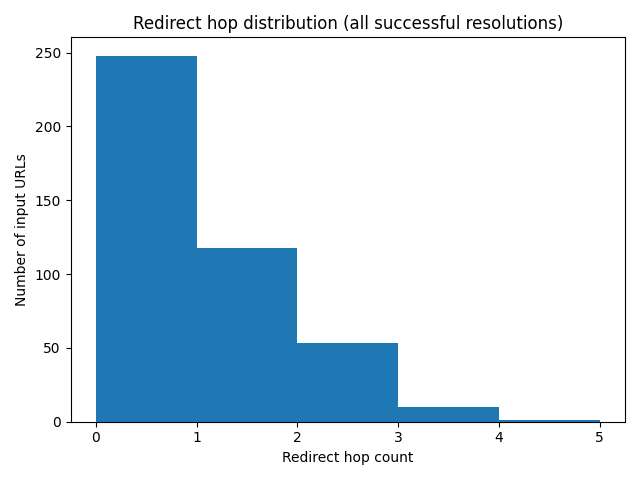
\includegraphics[width=\linewidth]{../results/ca/authorities/redirects/hop_distribution_all_success.png}
\captionof{figure}{This figure shows how many redirects the scanner had to follow from the initial input URL to reach a final response (of any status) for URLs that completed the redirect resolution without errors. A bar at 0 indicates URLs that returned a final response immediately without redirecting; a bar at 1 indicates URLs that performed exactly one redirect, and so on. This distribution gives a sense of how \emph{deep} typical redirect chains are in the studied population.
}
\label{fig:ca:auth:hop_all_success}
\end{minipage}
\end{center}

\begin{center}
\begin{minipage}{\plotwidth}
\centering
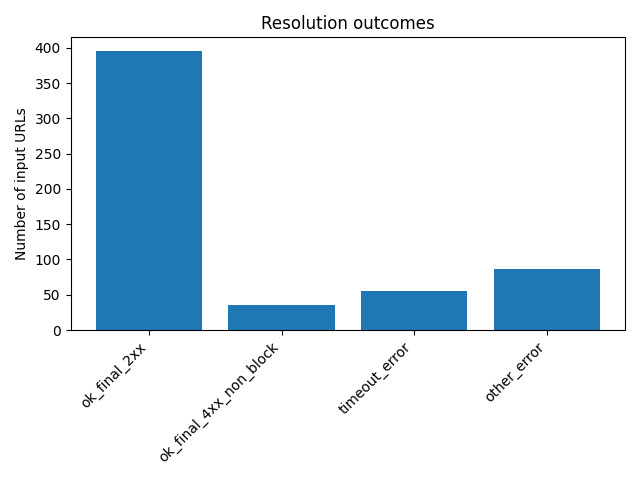
\includegraphics[width=\linewidth]{../results/ca/authorities/redirects/resolution_outcomes.png}
\captionof{figure}{Each bar corresponds to one high-level outcome category for the redirect resolution stage. ``ok\_final\_2xx'' indicates URLs where the scanner successfully followed redirects and obtained a 2xx response. ``blocked\_403\_503'' indicates URLs where at least one response in the resolution chain returned HTTP 403 or 503, suggesting the presence of a WAF or access control that blocked the scanner. ``timeout\_error'', ``redirect\_error'', and ``other\_error'' capture various error conditions. The relative bar heights show how often each outcome occurred.}
\label{fig:ca:auth:resolution_outcomes}
\end{minipage}
\end{center}

\begin{center}
\begin{minipage}{\plotwidth}
\centering
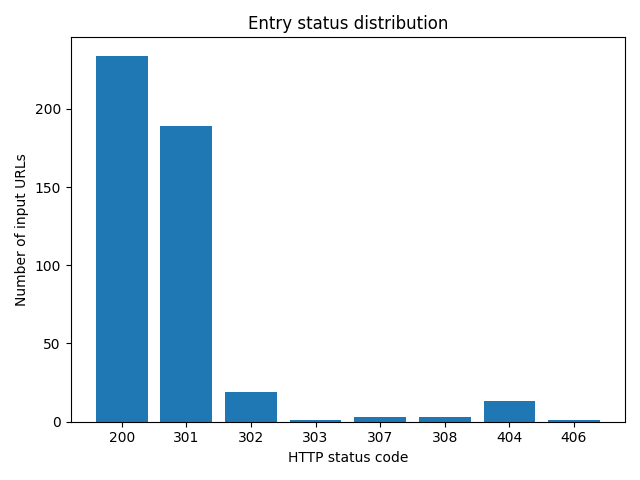
\includegraphics[width=\linewidth]{../results/ca/authorities/redirects/entry_status_distribution.png}
\captionof{figure}{
This figure shows the distribution of HTTP status codes for the final responses that the scanner received after resolving any redirects. It summarises how often sites eventually returned a success code (2xx), a redirect (3xx), a client error (4xx) such as 404 or 403, or a server error (5xx) such as 500 or 503. In combination with the entry status distribution, it reveals how often a URL ultimately succeeds even if the first response is a redirect or a soft error.
}
\label{fig:ca:auth:entry_status}
\end{minipage}
\end{center}


\begin{center}
\begin{minipage}{\plotwidth}
\centering
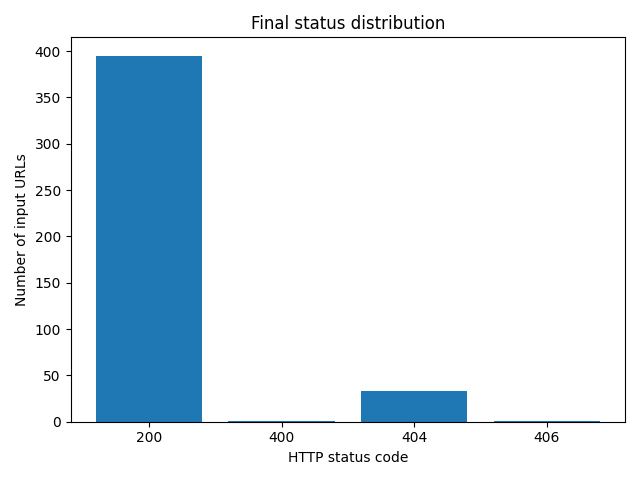
\includegraphics[width=\linewidth]{../results/ca/authorities/redirects/final_status_distribution.png}
\captionof{figure}{
This figure shows the distribution of HTTP status codes for the final responses that the scanner received after resolving any redirects. It summarises how often sites eventually returned a success code (2xx), a redirect (3xx), a client error (4xx) such as 404 or 403, or a server error (5xx) such as 500 or 503. In combination with the entry status distribution, it reveals how often a URL ultimately succeeds even if the first response is a redirect or a soft error. }
\label{fig:ca:auth:final_status}
\end{minipage}
\end{center}

\begin{center}
\begin{minipage}{\plotwidth}
\centering
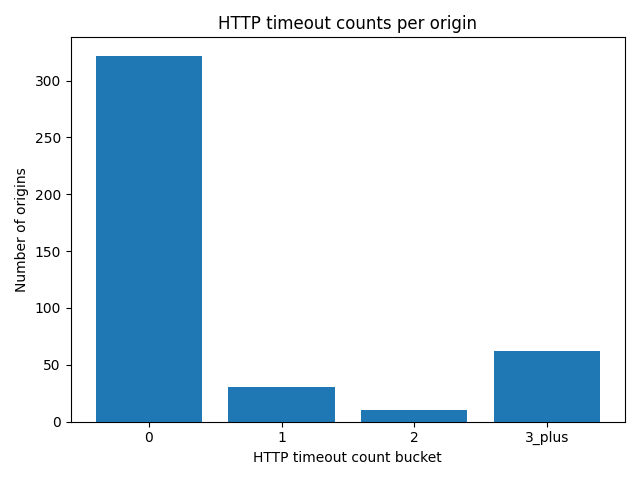
\includegraphics[width=\linewidth]{../results/ca/authorities/redirects/origin_http_timeout_buckets.png}
\captionof{figure}{This figure shows, for each origin, how many HTTP-level timeouts the scanner experienced during the entire scan, aggregated into buckets. Origins in the ``0'' bucket never timed out; those in``3\_plus'' produced three or more HTTP timeouts, indicating sites that were repeatedly unreachable or unreliable during the scan window.}
\label{fig:ca:auth:http_timeout}
\end{minipage}
\end{center}

\begin{center}
\begin{minipage}{\plotwidth}
\centering
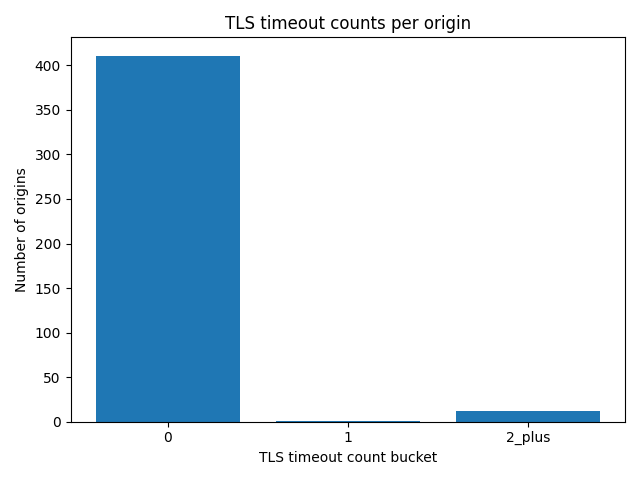
\includegraphics[width=\linewidth]{../results/ca/authorities/redirects/origin_tls_timeout_buckets.png}
\captionof{figure}{This figure shows how many TLS handshake timeouts the scanner encountered per origin, bucketed into 0, 1, and 2-or-more timeouts. Origins in the ``2\_plus'' bucket systematically failed to complete the TLS handshake, which may correspond to misconfigured servers, aggressive WAF behaviour, or transient network issues.}
\label{fig:ca:auth:tls_timeout}
\end{minipage}
\end{center}
  
\begin{center}
\begin{minipage}{\plotwidth}
\centering
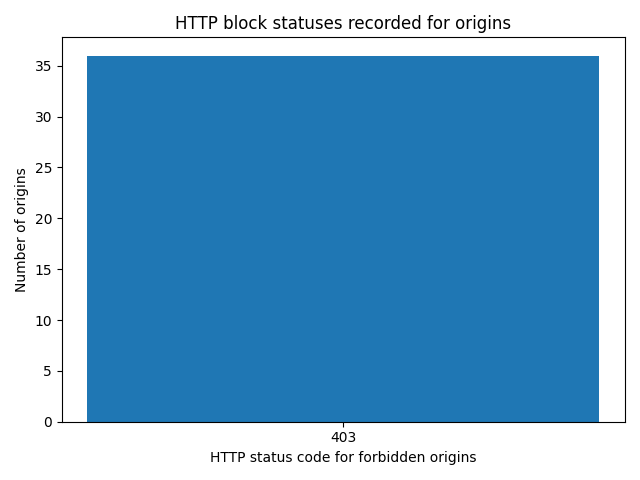
\includegraphics[width=\linewidth]{../results/ca/authorities/redirects/origin_http_forbidden_statuses.png}
\captionof{figure}{This figure shows which HTTP status codes are associated with origins that the scanner marked as http\_forbidden. For each origin where the scanner concluded that HTTP access was forbidden, we recorded any HTTP status codes returned (typically 403 or 503). The bars indicate how many origins produced 403 Forbidden responses, how many produced 503 Service Unavailable responses, and how many produced other status codes. This helps characterise the kinds of blocking or WAF behaviour we encountered at the origin level.}
\label{fig:ca:auth:forbidden_status}
\end{minipage}
\end{center}


\paragraph*{HTTPS/HSTS Connectivity \& Redirection}

\begin{center}
\begin{minipage}{\plotwidth}
\centering
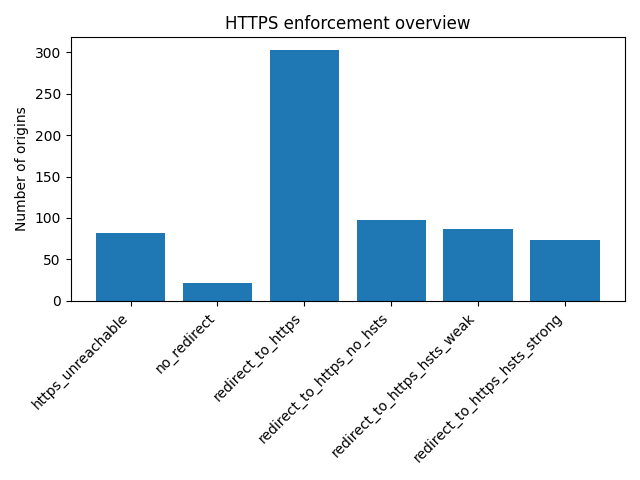
\includegraphics[width=\linewidth]{../results/ca/authorities/hsts_https/https_enforcement_overview.png}
\captionof{figure}{Overview of HTTPS enforcement outcomes per origin. For each origin we combine the \texttt{https\_connectivity} and HSTS module results and count: (i) \emph{https\_unreachable}, where neither module recorded a successful HTTPS response; (ii) \emph{no\_redirect}, where the HTTP probe to \texttt{http://origin/} returned a non--3xx status code and therefore did not redirect to HTTPS; (iii) \emph{redirect\_to\_https}, where the HTTP probe returned a 3xx status and the Location header pointed to an HTTPS URL; and the three nested subsets \emph{redirect\_to\_https\_no\_hsts}, \emph{redirect\_to\_https\_hsts\_weak}, and \emph{redirect\_to\_https\_hsts\_strong}, which further restrict \emph{redirect\_to\_https} to sites whose HTTPS response respectively (a) omits HSTS entirely, (b) sets HSTS but with max-age $<$ 1 year or without \texttt{includeSubDomains}, or (c) sets ``strong'' HSTS with max-age~$\geq$~1~year and \texttt{includeSubDomains}.}
\label{fig:ca:auth:https_enforcement_overview}
\end{minipage}
\end{center}

\begin{center}
\begin{minipage}{\plotwidth}
\centering
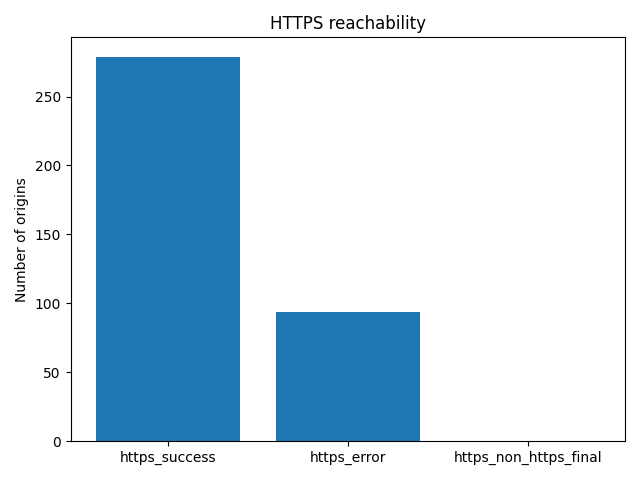
\includegraphics[width=\linewidth]{../results/ca/authorities/hsts_https/https_reachability.png}
\captionof{figure}{HTTPS reachability as reported by the \texttt{https\_connectivity} module. Each origin is classified as \emph{https\_success} if the module completed the request with \texttt{success{=}True} and a final HTTPS scheme; \emph{https\_error} if HTTPS was attempted but the row contains a non-empty error string (for example, timeout or client error) and \texttt{success{=}False}; or \emph{https\_non\_https\_final} if the request completed without an explicit error but the recorded final scheme was not HTTPS. Bar heights represent the number of origins in each category.}
\label{fig:ca:auth:https_reachable}
\end{minipage}
\end{center}


\begin{center}
  \begin{minipage}{\plotwidth}
  \centering
  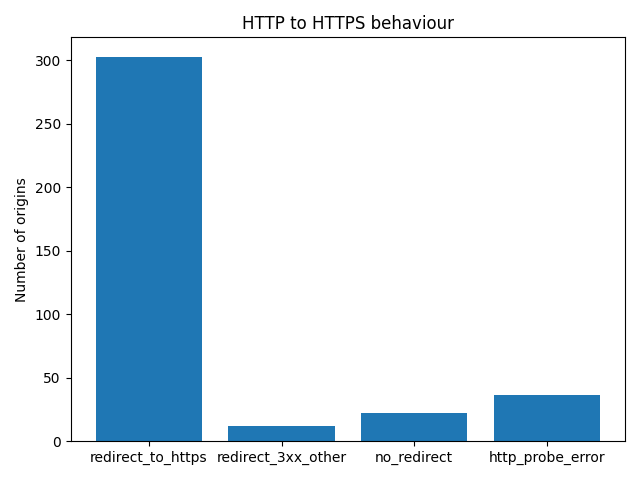
\includegraphics[width=\linewidth]{../results/ca/authorities/hsts_https/http_to_https_behaviour.png}
  \captionof{figure}{Behaviour of \texttt{http://origin/} requests as observed by the HSTS module. For each origin we count: \emph{redirect\_to\_https}, where the HTTP probe returned a 3xx status code and the Location header pointed to an HTTPS URL; \emph{redirect\_3xx\_other}, where the status code was 3xx but the redirect target was not HTTPS; \emph{no\_redirect}, where the HTTP probe succeeded but returned a non--3xx status code (for example, a 200 or 4xx served over HTTP); and \emph{http\_probe\_error}, where no HTTP status code was recorded because the probe failed or timed out before any response.}
  \label{fig:ca:auth:http_to_https_behaviour}
  \end{minipage}
  \end{center}
  
\begin{center}
  \begin{minipage}{\plotwidth}
  \centering
  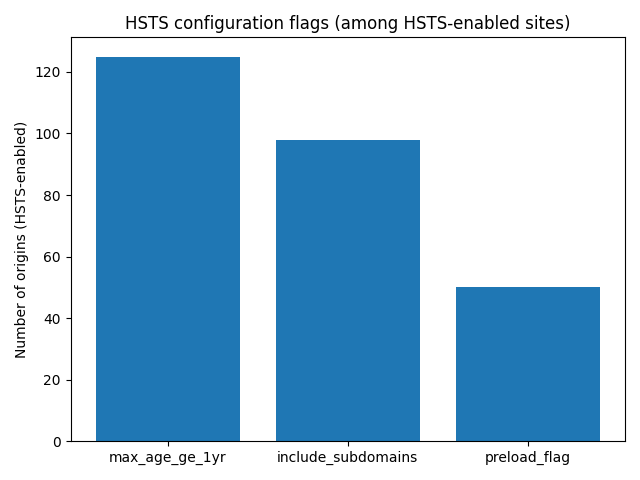
\includegraphics[width=\linewidth]{../results/ca/authorities/hsts_https/hsts_flags_among_hsts_sites.png}
  \captionof{figure}{Configuration of HSTS flags among origins that set any HSTS header. We first restrict to origins where the HSTS module marked \texttt{https\_ok{=}True} and \texttt{has\_hsts{=}True}. Among this HSTS-enabled subset we count how many also configured (i) a \texttt{max-age} directive of at least one year (\texttt{max\_age\_ge\_1yr}), (ii) the \texttt{includeSubDomains} directive, and (iii) the \texttt{preload} directive. Bar heights therefore represent how often each strengthening flag appears among sites that already deploy HSTS.}
  \label{fig:ca:auth:hsts_flags}
  \end{minipage}
  \end{center}


\begin{center}
\begin{minipage}{\plotwidth}
\centering
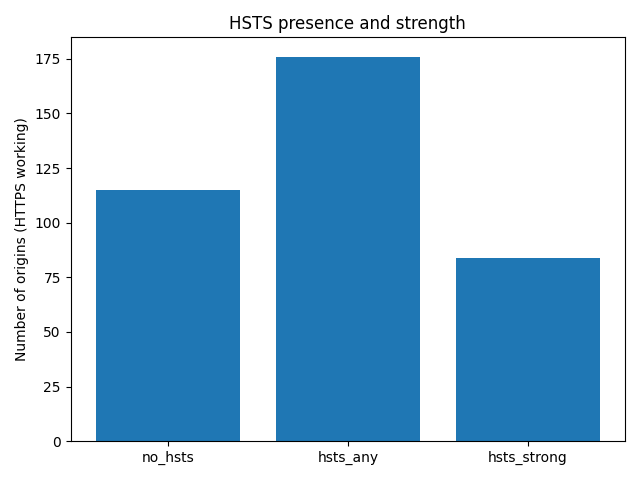
\includegraphics[width=\linewidth]{../results/ca/authorities/hsts_https/hsts_presence_and_strength.png}
\captionof{figure}{HSTS presence and strength among origins whose HTTPS response succeeded. We first restrict to origins where the HSTS module recorded \texttt{https\_ok{=}True}. Within this set, \emph{no\_hsts} counts sites that did not send a Strict-Transport-Security header; \emph{hsts\_any} counts all sites that did; and \emph{hsts\_strong} counts the subset that configured both \texttt{max-age}~$\geq$~1~year and \texttt{includeSubDomains} (our ``strong HSTS'' baseline).}
\label{fig:ca:auth:hsts_presence}
\end{minipage}
\end{center}

\paragraph*{TLS \& Cipher Suites}

\begin{center}
  \begin{minipage}{\plotwidth}
  \centering
  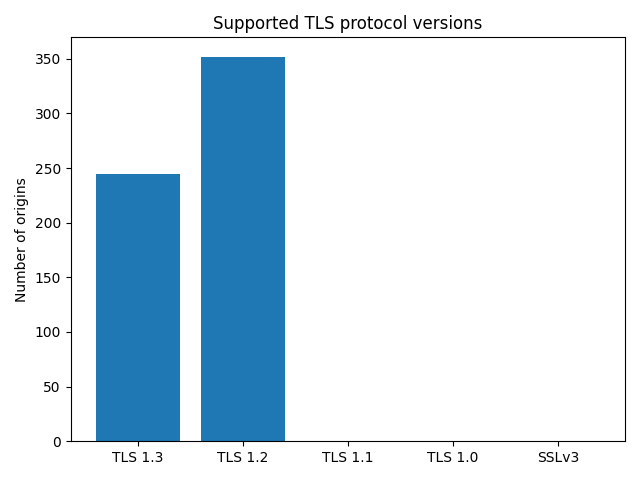
\includegraphics[width=\linewidth]{../results/ca/authorities/tls_cipher/tls_protocol_support.png}
  \captionof{figure}{Support for individual TLS protocol versions. Using the TLS module, we attempt separate handshakes at TLS~1.3, TLS~1.2, TLS~1.1, TLS~1.0, and SSLv3. For each version, the bar height shows how many origins completed a handshake at that exact version (the corresponding field \texttt{tls13}, \texttt{tls12}, \texttt{tls11}, \texttt{tls10}, or \texttt{ssl\_legacy} was \texttt{True}).}
  \label{fig:ca:auth:tls_protocol_support}
  \end{minipage}
  \end{center}

 % This chart is redundant
  % \begin{center}
  %   \begin{minipage}{\plotwidth}
  %   \centering
  %   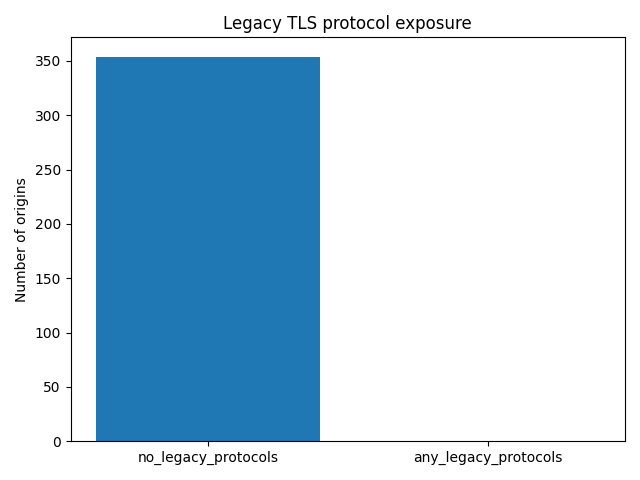
\includegraphics[width=\linewidth]{../results/ca/authorities/tls_cipher/legacy_protocol_exposure.png}
  %   \captionof{figure}{Legacy TLS protocol exposure. For each origin we check whether any legacy protocol (TLS~1.1, TLS~1.0, or SSLv3) was successfully negotiated. Origins that support none of these are counted as \emph{no\_legacy\_protocols}; origins that support at least one are counted as \emph{any\_legacy\_protocols}. This highlights how many sites have fully disabled deprecated versions versus still accepting them.}
  %   \label{fig:ca:auth:htsts_flags}
  %   \end{minipage}
  %   \end{center}
  
\begin{center}
\begin{minipage}{\plotwidth}
\centering
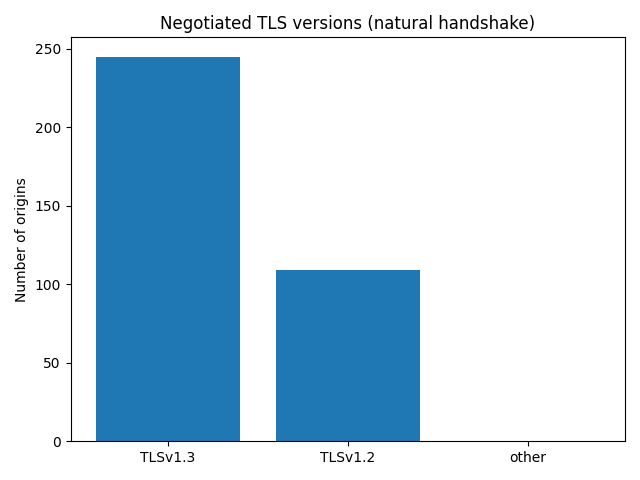
\includegraphics[width=\linewidth]{../results/ca/authorities/tls_cipher/negotiated_tls_versions.png}
\captionof{figure}{Negotiated TLS versions for the natural client handshake. The cipher module records the \texttt{negotiated\_version} reported by the TLS library when connecting without forcing a specific protocol version. Bars show how many origins negotiated TLS~1.3, TLS~1.2, or another/unspecified version (\emph{other}) under this normal connection profile.}
\label{fig:ca:auth:natural_tls_version}
\end{minipage}
\end{center}

% This chart also might be redundant, I think nearly all TLS 1.3 cipher suites are are "recommended". 
\begin{center}
\begin{minipage}{\plotwidth}
\centering
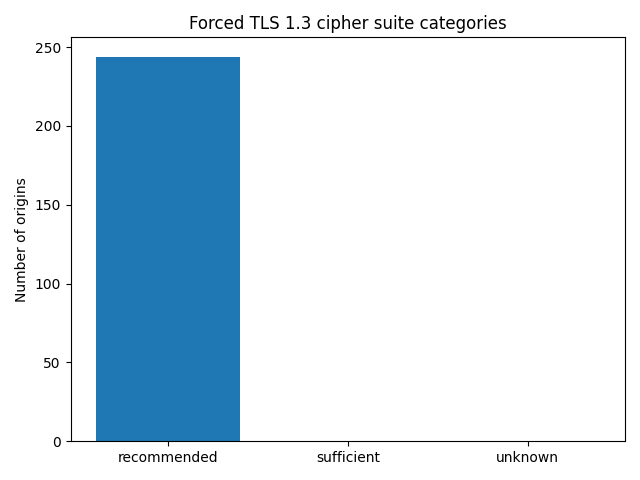
\includegraphics[width=\linewidth]{../results/ca/authorities/tls_cipher/tls13_cipher_categories.png}
\captionof{figure}{Cipher suite categories for forced TLS~1.3 handshakes. For each origin where a TLS~1.3 handshake succeeded, the cipher module records the chosen cipher suite and assigns a category: \emph{recommended} if it appears in the CCCS recommended TLS~1.3 list, \emph{sufficient} if it appears in a secondary acceptable list, and \emph{unknown} otherwise. Bar heights indicate how many origins fell into each category.}
\label{fig:ca:auth:tls13_cipher_categories}
\end{minipage}
\end{center}
    
\begin{center}
\begin{minipage}{\plotwidth}
\centering
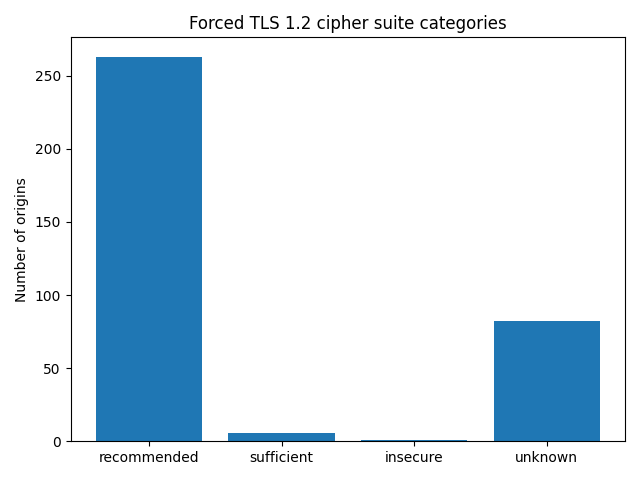
\includegraphics[width=\linewidth]{../results/ca/authorities/tls_cipher/tls12_cipher_categories.png}
\captionof{figure}{Cipher suite categories for forced TLS~1.2 handshakes. For origins where a TLS~1.2 handshake succeeded, the cipher module classifies the negotiated cipher suite as \emph{recommended} (modern AEAD/ECDHE suites), \emph{sufficient}, \emph{insecure} (RC4, 3DES, SHA--1, or other legacy families), or \emph{unknown}. Bars show how many origins negotiated a cipher in each category when TLS~1.2 was forced.}
\label{fig:ca:auth:tls12_cipher_categories}
\end{minipage}
\end{center}
  
\begin{center}
\begin{minipage}{\plotwidth}
\centering
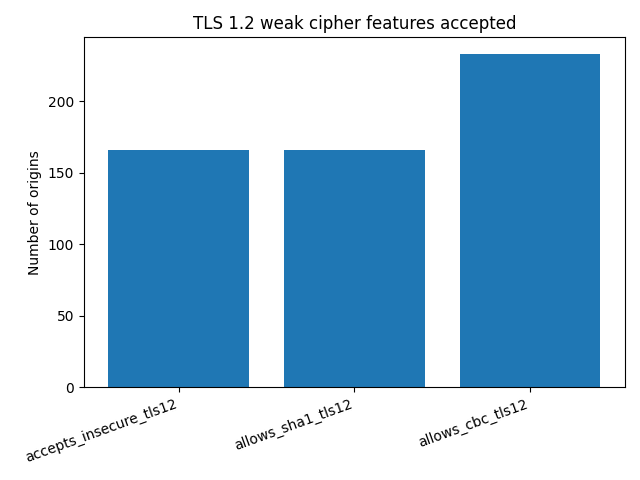
\includegraphics[width=\linewidth]{../results/ca/authorities/tls_cipher/tls12_weak_features.png}
\captionof{figure}{Acceptance of weak TLS~1.2 cipher features. Using targeted probes, the cipher module tests whether a server will negotiate (i) any cipher from an explicitly insecure bundle sourced from the NSA, (ii) SHA--1 based cipher suites only (\texttt{allows\_sha1\_tls12}), or (iii) CBC-mode cipher suites only (\texttt{allows\_cbc\_tls12}). Each bar counts the number of origins for which the corresponding probe succeeded (\texttt{True}), indicating that the server is still willing to accept that class of weak TLS~1.2 configuration.}
\label{fig:ca:auth:tls12_weak_features}
\end{minipage}
\end{center}

\paragraph*{Security.txt}

\begin{center}
\begin{minipage}{\plotwidth}
\centering
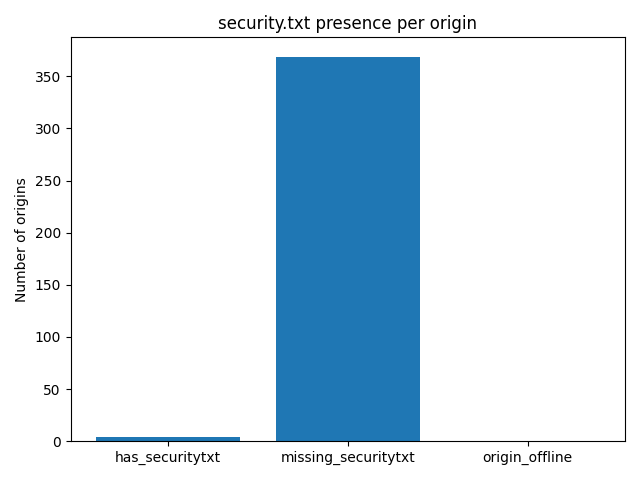
\includegraphics[width=\linewidth]{../results/ca/authorities/securitytxt/securitytxt_presence.png}
\captionof{figure}{Deployment of \texttt{security.txt} per origin. The scanner records three outcomes: \emph{has\_securitytxt}, where at least one usable \texttt{security.txt} file was found at \texttt{/.well-known/security.txt} or \texttt{/security.txt} and contained a \texttt{Contact} or \texttt{Expires} field; \emph{missing\_securitytxt}, where the origin was reachable but no such file was found; and \emph{origin\_offline}, where the origin was marked offline and the module did not probe for \texttt{security.txt}. Bar heights show the number of origins in each category.}
\label{fig:ca:auth:securitytxt_presence}
\end{minipage}
\end{center}
  

\begin{center}
\begin{minipage}{\plotwidth}
\centering
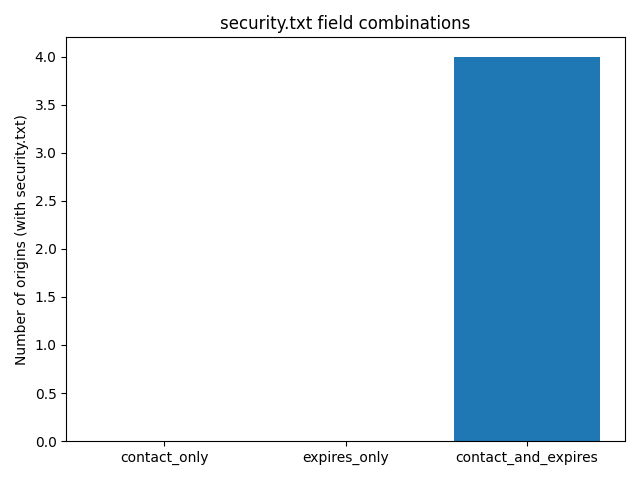
\includegraphics[width=\linewidth]{../results/ca/authorities/securitytxt/securitytxt_field_combinations.png}
\captionof{figure}{Field combinations observed in deployed \texttt{security.txt} files. Among origins where \texttt{security.txt} was present, we classify each file as \emph{contact\_only} (at least one \texttt{Contact} field but no \texttt{Expires}), \emph{expires\_only} (an \texttt{Expires} field but no \texttt{Contact}), or \emph{contact\_and\_expires} (both fields present). Counts are per origin, not per file, and show how often each minimal disclosure combination appears.}
\label{fig:ca:auth:securitytxt_field}
\end{minipage}
\end{center}

\begin{center}
\begin{minipage}{\plotwidth}
\centering
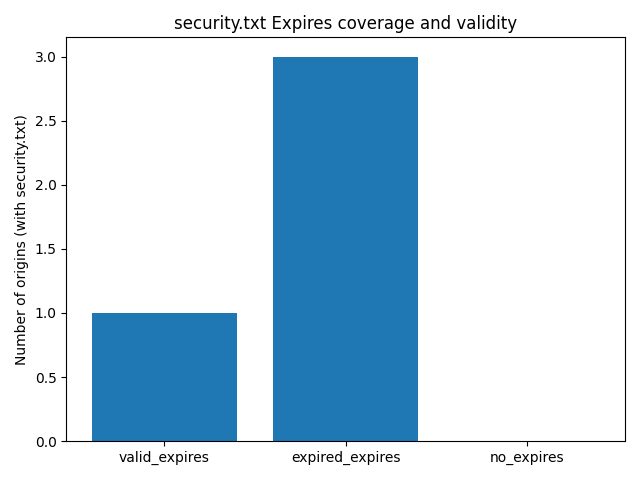
\includegraphics[width=\linewidth]{../results/ca/authorities/securitytxt/securitytxt_expires_validity.png}
\captionof{figure}{Coverage and freshness of the \texttt{Expires} field in \texttt{security.txt}. For origins with \texttt{security.txt} present, we separate files into three groups: \emph{valid\_expires}, where a syntactically valid \texttt{Expires} value was parsed and remained in the future at scan time; \emph{expired\_expires}, where \texttt{Expires} was present but already in the past; and \emph{no\_expires}, where the file contained no \texttt{Expires} field at all.}
\label{fig:ca:auth:securitytxt_expires}
\end{minipage}
\end{center}

\begin{center}
\begin{minipage}{\plotwidth}
\centering
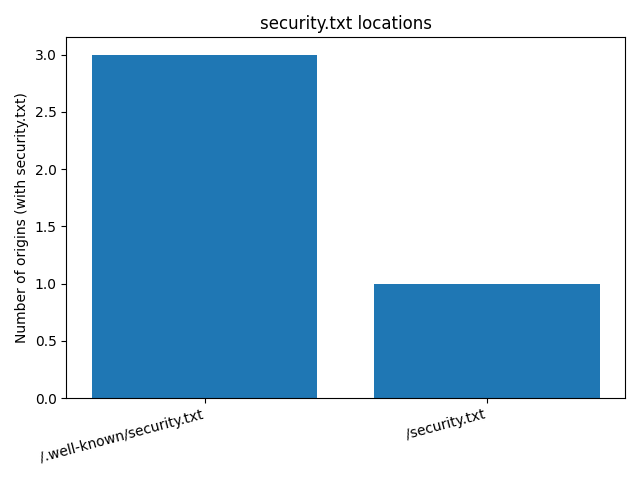
\includegraphics[width=\linewidth]{../results/ca/authorities/securitytxt/securitytxt_locations.png}
\captionof{figure}{Locations used for \texttt{security.txt}. Among origins that deployed a usable \texttt{security.txt} file, we count how many placed it at the RFC~9116-recommended path \texttt{/.well-known/security.txt} versus the legacy fallback \texttt{/security.txt}. Each bar corresponds to one path and reports the number of origins using it.}
\label{fig:ca:auth:securitytxt_location}
\end{minipage}
\end{center}

\begin{center}
\begin{minipage}{\plotwidth}
\centering
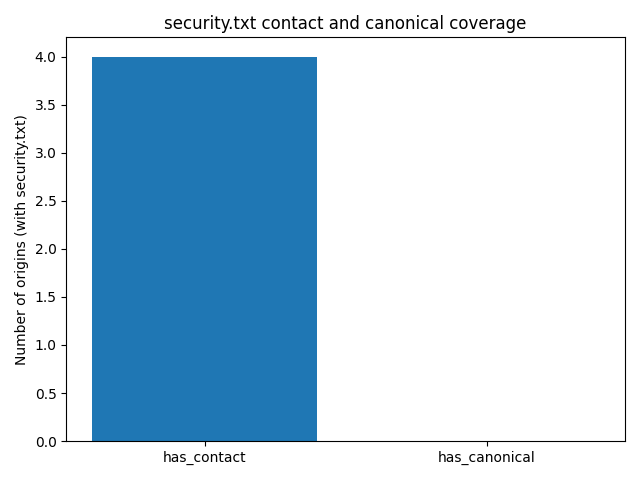
\includegraphics[width=\linewidth]{../results/ca/authorities/securitytxt/securitytxt_contact_canonical.png}
\captionof{figure}{Contact and canonical information advertised via \texttt{security.txt}. Among origins with a present \texttt{security.txt} file, the \emph{has\_contact} bar counts files that expose at least one \texttt{Contact} field (for example, an email address or URL for reporting vulnerabilities), while the \emph{has\_canonical} bar counts files that include at least one \texttt{Canonical} URL pointing to the authoritative copy of their disclosure policy. Bars are counts of origins, not individual fields.}
\label{fig:ca:auth:securitytxt_contact}
\end{minipage}
\end{center}

\paragraph*{Error Leaks}


\begin{center}
\begin{minipage}{\plotwidth}
\centering
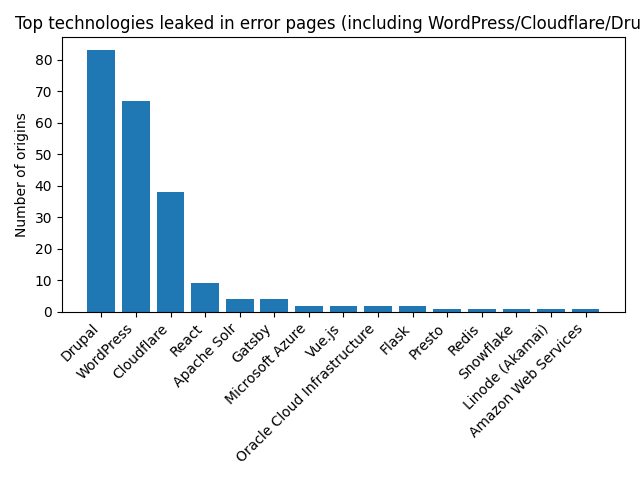
\includegraphics[width=\linewidth]{../results/ca/authorities/error_leak/error_leak_tech_topN_all.png}
\captionof{figure}{Top technologies disclosed by error pages. For each origin, the scanner sends a request to a randomly generated non-existent path and inspects the resulting error page for framework, database, and cloud-platform signatures using regular expressions. After filtering out technologies in an explicit ignore list (for example, \texttt{Next.js}, which produced many false positives), we count how many origins leak each \texttt{tech\_name}. Bars show the top $N$ technologies by number of origins, including major platforms such as WordPress, Cloudflare, and Drupal.}
\label{fig:ca:auth:error_leak_top_N_all}
\end{minipage}
\end{center}
  

\begin{center}
\begin{minipage}{\plotwidth}
\centering
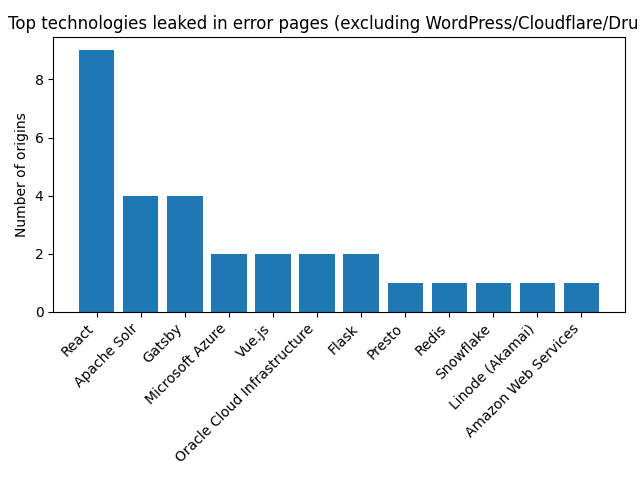
\includegraphics[width=\linewidth]{../results/ca/authorities/error_leak/error_leak_tech_topN_no_wp_cf_drupal.png}
\captionof{figure}{Second-tier technologies leaked by error pages (excluding WordPress, Cloudflare, and Drupal). Using the same detection method as in the previous figure, we remove the three most common platform signatures and re-rank the remaining technologies. Each bar reports how many origins had error pages that mentioned the corresponding framework or component at least once. This highlights less prominent but still widely deployed stacks exposed through error handling.}
\label{fig:ca:auth:error_leak_top_N_wo_big_guys}
\end{minipage}
\end{center}


\begin{center}
\begin{minipage}{\plotwidth}
\centering
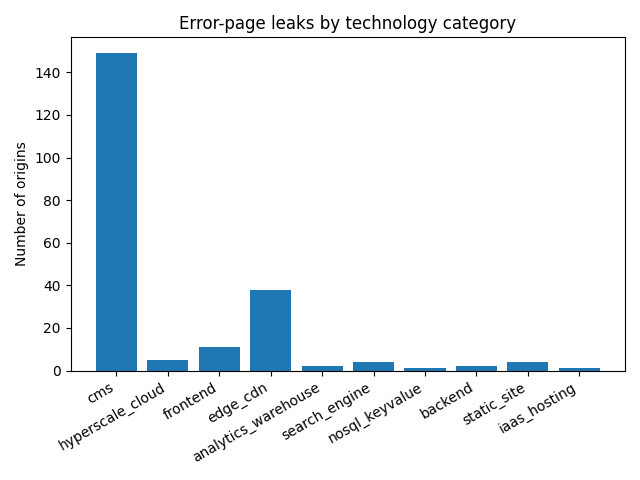
\includegraphics[width=\linewidth]{../results/ca/authorities/error_leak/error_leak_category_distribution.png}
\captionof{figure}{Error-page leaks by technology category. Each \texttt{error\_leak} match is labelled with a high-level category (for example, framework, database, cloud platform). For every category, we count how many distinct origins leaked at least one technology in that group. Bars therefore represent the number of sites whose error pages reveal something about their application framework, backing database, hosting platform, or other internal components.}
\label{fig:ca:auth:error_leak_cat_distribution}
\end{minipage}
\end{center}

\paragraph*{Headers: Security \& Revealing}

\begin{center}
\begin{minipage}{\plotwidth}
\centering
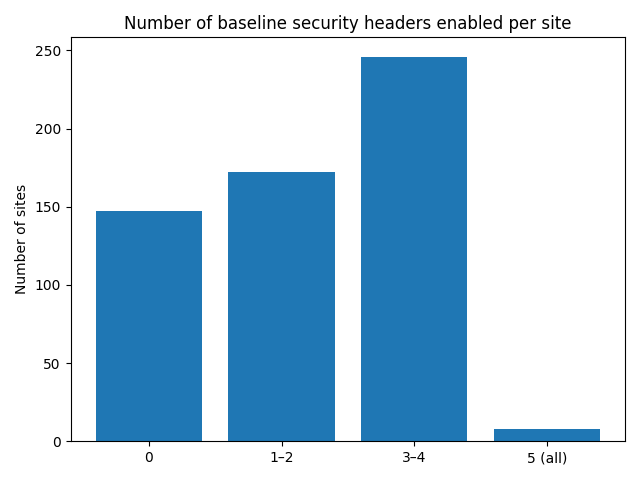
\includegraphics[width=\linewidth]{../results/ca/authorities/headers/headers_baseline_coverage.png}
\captionof{figure}{
Distribution of how many core browser-side security headers each site enabled.
For every origin, the scanner's \texttt{headers} module inspects the final HTTP
response and classifies five ``baseline'' protections: \texttt{Referrer-Policy},
CSP \texttt{frame-ancestors}, \texttt{X-Frame-Options}, \texttt{X-Content-Type-Options},
and \texttt{Permissions-Policy}. A header is counted as ``enabled'' if its rating
is either \emph{recommended} or \emph{sufficient} according to OWASP/MDN-inspired
rules in the classifier. Each site is placed into one of four buckets based on how
many of these five protections are enabled (0, 1--2, 3--4, or all 5). The height
of each bar shows how many sites fall into that bucket, so taller bars indicate
that configuration pattern is more common.}
\label{fig:ca:auth:headers_baseline}
\end{minipage}
\end{center}
  

\begin{center}
  \begin{minipage}{\plotwidth}
  \centering
  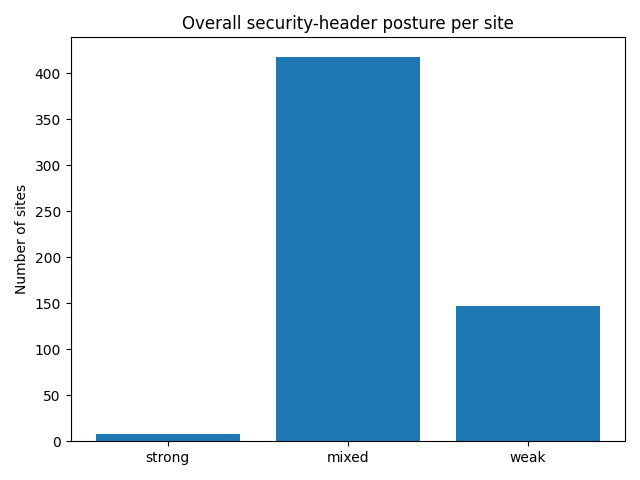
\includegraphics[width=\linewidth]{../results/ca/authorities/headers/headers_posture_bucket.png}
  \captionof{figure}{
Overall security-header posture of each site. Using the same five baseline
headers as in Figure~\ref{fig:headers_baseline}, the scanner counts how
many are rated \emph{recommended} or \emph{sufficient} and also notes whether
any are rated \emph{insecure} or \emph{obsolete}. A site is labelled
\emph{strong} if at least three baseline headers are recommended or sufficient
and none are insecure/obsolete, \emph{weak} if none of the five are
recommended/sufficient, and \emph{mixed} otherwise (some protections present,
but at least one header misconfigured or missing). Each bar reports how many
sites fall into each posture category. Reading from left to right therefore
shows how many sites have broadly good, partial, or weak browser-side header
configurations.}
  \label{fig:ca:auth:headers_posture_bucket}
  \end{minipage}
  \end{center}
  

\begin{center}
\begin{minipage}{\plotwidth}
\centering
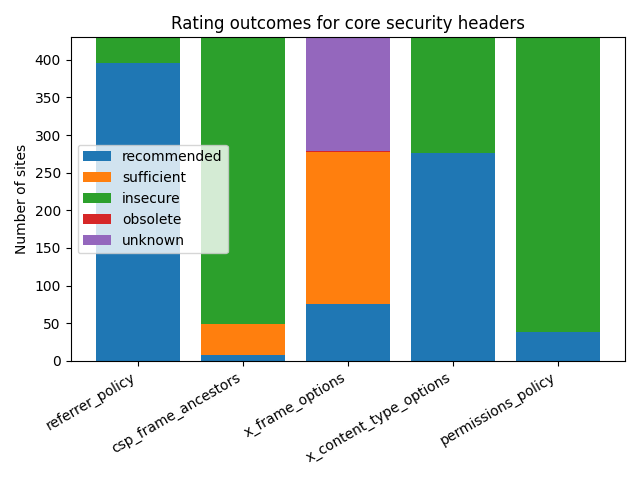
\includegraphics[width=\linewidth]{../results/ca/authorities/headers/headers_security_rule_ratings.png}
\captionof{figure}{
Rating outcomes for each core security header rule. For every site and every
rule (\texttt{referrer\_policy}, CSP \texttt{frame\_ancestors},
\texttt{X-Frame-Options}, \texttt{X-Content-Type-Options}, and
\texttt{Permissions-Policy}), the \texttt{headers} module applies a rule-specific
classifier and assigns one of five ratings: \emph{recommended}, \emph{sufficient},
\emph{insecure}, \emph{obsolete}, or \emph{unknown}. For each rule, we then count
how many sites received each rating and stack those counts into a single bar.
Within each bar, the height of each coloured segment shows the number of sites
with that outcome, and the total bar height equals the number of sites analysed.
Bars dominated by blue/orange segments indicate that the corresponding header is
usually configured well; bars dominated by green/red show headers that are
typically missing or misconfigured.}
\label{fig:ca:auth:headers_ratings}
\end{minipage}
\end{center}

\begin{center}
\begin{minipage}{\plotwidth}
\centering
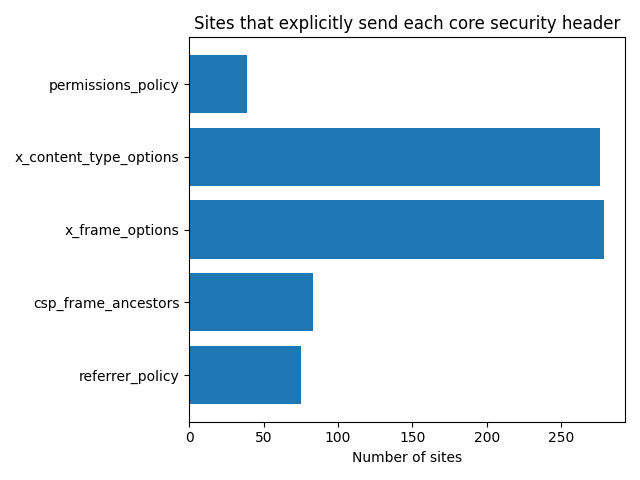
\includegraphics[width=\linewidth]{../results/ca/authorities/headers/headers_security_header_presence.png}
\captionof{figure}{
Explicit use of each core security header. For each site and each baseline
header rule, the scanner records whether the corresponding HTTP header is
actually present in the final response (\texttt{present = True}). This figure
counts, for each rule, the number of sites that explicitly send that header,
regardless of how it is configured. Missing headers may still receive a rating
via the classifier's \texttt{on\_missing\_class} default, but are not counted in
these bars. The horizontal axis shows how many sites send each header, so longer
bars indicate protections that are explicitly configured by most sites, while
shorter bars highlight headers that are rarely used in practice.}
\label{fig:ca:auth:headers_security_presence}
\end{minipage}
\end{center}
  

\begin{center}
\begin{minipage}{\plotwidth}
\centering
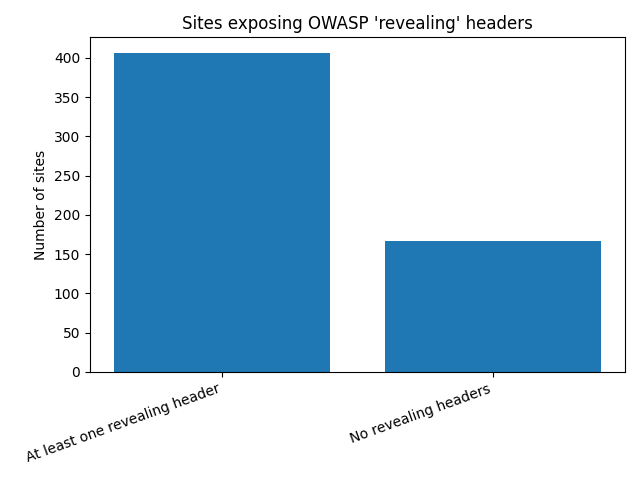
\includegraphics[width=\linewidth]{../results/ca/authorities/headers/headers_revealing_any.png}
\captionof{figure}{
Presence of OWASP ``revealing'' headers per site. The \texttt{headers} module
checks each final response for a list of information-leaking headers (for
example \texttt{Server}, \texttt{X-Powered-By}, \texttt{X-Generator} and similar
banners identified by OWASP as candidates for removal). A site is placed in the
``At least one revealing header'' group if any of these headers are present,
otherwise it is placed in the ``No revealing headers'' group. Each bar shows how
many sites fall into each category. Reading this figure indicates what fraction
of sites expose at least one stack-identifying header versus those that suppress
such banners entirely.}
\label{fig:ca:auth:headers_revealing_any}
\end{minipage}
\end{center}
  

\begin{center}
\begin{minipage}{\plotwidth}
\centering
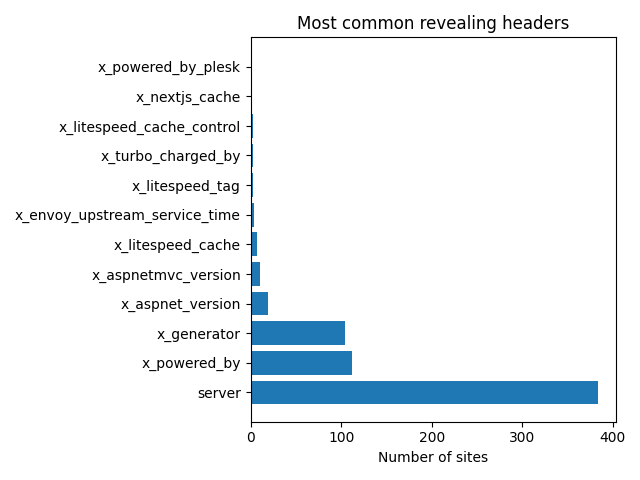
\includegraphics[width=\linewidth]{../results/ca/authorities/headers/headers_revealing_topN.png}
\captionof{figure}{
Most common revealing headers across all sites. For every site that exposes at
least one OWASP ``revealing'' header, the scanner records which header names
were present (for example, \texttt{server}, \texttt{x\_powered\_by},
\texttt{x\_generator}). This figure selects the top $N$ header names by the
number of sites that use them and plots those counts as horizontal bars. The
length of each bar shows how many sites include that particular header in their
final response. Reading from top to bottom reveals which banners---such as
generic \texttt{Server} strings or specific framework identifiers---are most
widely exposed to the internet.}
\label{fig:ca:auth:headers_revealing_topN}
\end{minipage}
\end{center}
    

\begin{center}
\begin{minipage}{\plotwidth}
\centering
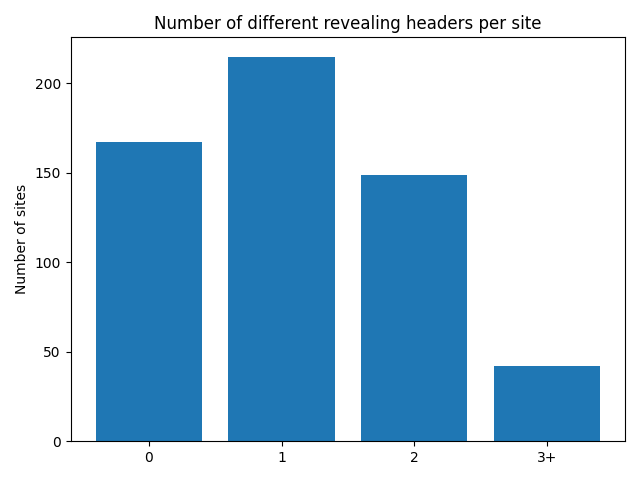
\includegraphics[width=\linewidth]{../results/ca/authorities/headers/headers_revealing_count_distribution.png}
\captionof{figure}{
Number of distinct revealing headers exposed per site. For each origin, the
scanner counts how many different revealing header types (from the OWASP list)
are present in the final response. Sites are then grouped into buckets with 0,
1, 2, or 3-or-more such headers. The height of each bar shows how many sites
fall into that bucket. This chart therefore indicates not only whether sites
leak stack information via headers at all, but also how verbose their banners
are---for example, whether they expose multiple overlapping identifiers (such as
\texttt{Server} plus \texttt{X-Powered-By} plus \texttt{X-Generator}) or none.}
\label{fig:ca:auth:headers_revealing_count_distribution}
\end{minipage}
\end{center}


\begin{center}
\begin{minipage}{\plotwidth}
\centering
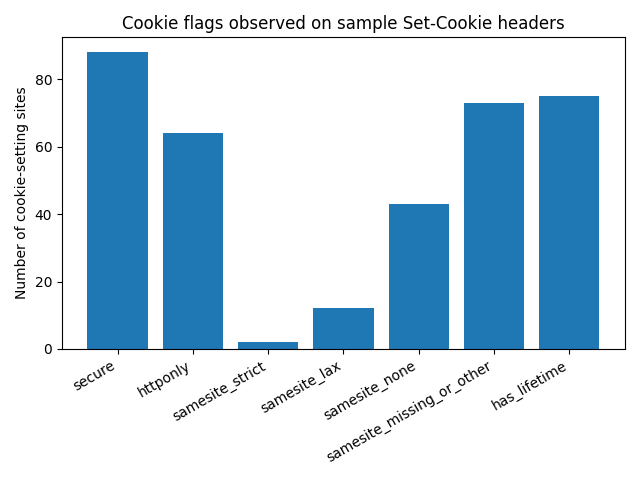
\includegraphics[width=\linewidth]{../results/ca/authorities/headers/headers_cookies_flags.png}
\captionof{figure}{
Cookie flag usage on sites that set cookies. The \texttt{headers} module
aggregates information from the final response's \texttt{Set-Cookie} headers and
classifies a sample cookie per site. This figure considers only sites that set
at least one cookie and, for that sample cookie, counts how many sites used each
flag: \texttt{Secure}, \texttt{HttpOnly}, which \texttt{SameSite} value
(\texttt{Strict}, \texttt{Lax}, \texttt{None}, or missing/other), and whether a
lifetime was explicitly specified via \texttt{Max-Age} or \texttt{Expires}. Each
bar shows the number of cookie-setting sites where the corresponding attribute
was present. Reading across the bars reveals how common it is for session
cookies to be protected against network theft (Secure), script access
(HttpOnly), cross-site attacks (SameSite), and long-lived persistence
(explicit lifetime).}
\label{fig:ca:auth:headers_cookies_flags}
\end{minipage}
\end{center}

\begin{center}
\begin{minipage}{\plotwidth}
\centering
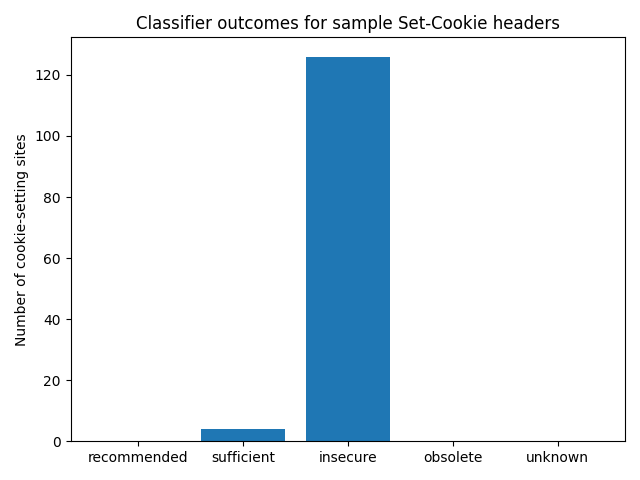
\includegraphics[width=\linewidth]{../results/ca/authorities/headers/headers_cookies_ratings.png}
\captionof{figure}{
Classifier outcomes for sample cookies on cookie-setting sites. For every site
that sends at least one \texttt{Set-Cookie} header, the scanner applies a
rule-based classifier to a sample cookie and assigns one of several ratings:
\emph{recommended} (Secure + HttpOnly + SameSite=Strict),
\emph{sufficient} (Secure + HttpOnly + SameSite=Lax), \emph{insecure} (missing
one or more of these protections), or other categories such as \emph{unknown}.
This figure counts how many cookie-setting sites fall into each rating. The
height of each bar therefore indicates how often session cookies are configured
in a strongly locked-down way versus partially protected or weakly configured.}
\label{fig:ca:auth:headers_cookies_ratings}
\end{minipage}
\end{center}

% CA authorities had no stack traces
% \begin{center}
% \begin{minipage}{\plotwidth}
% \centering
% \includegraphics[width=\linewidth]{../results/ca/authorities/error_leak/error_leak_stacktrace_topN.png}
% \captionof{figure}{Top stack-trace language families exposed on error pages. The scanner searches error responses for language-specific stack-trace patterns (for example, Python \texttt{Traceback}, Java \texttt{Exception in thread}, PHP \texttt{Stack trace:}, or JavaScript \texttt{Error:} frames). After applying an explicit ignore list (currently empty), we count how many origins leaked at least one stack trace for each language family (displayed as \texttt{display\_name}, such as ``JavaScript / Node.js'' or ``C\# / .NET''). Bars show the top $N$ language families by number of affected origins.}
% \label{fig:ca:auth:error_leak_cat_distribution}
% \end{minipage}
% \end{center}
  

% \textbf{Educational Institutions}
% \begin{center}
% \begin{minipage}{\plotwidth}
% \centering
% 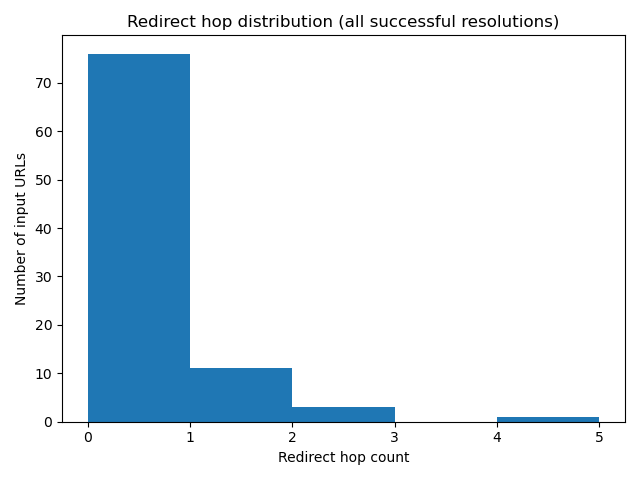
\includegraphics[width=\linewidth]{../results/ca/edu/redirects/hop_distribution_all_success.png}
% \captionof{figure}{This figure shows how many redirects the scanner had to follow from the initial input URL to reach a final response (of any status) for URLs that completed the redirect resolution without errors. A bar at 0 indicates URLs that returned a final response immediately without redirecting; a bar at 1 indicates URLs that performed exactly one redirect, and so on. This distribution gives a sense of how \emph{deep} typical redirect chains are in the studied population.
% }
% \label{fig:ca:edu:hop_all_success}
% \end{minipage}
% \end{center}

% \begin{center}
% \begin{minipage}{\plotwidth}
% \centering
% 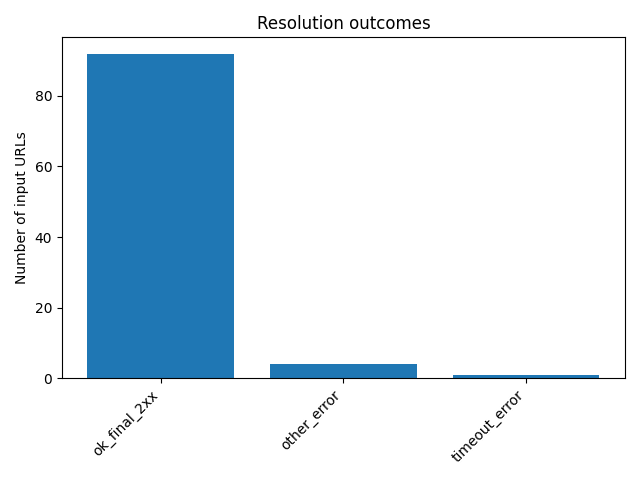
\includegraphics[width=\linewidth]{../results/ca/edu/redirects/resolution_outcomes.png}
% \captionof{figure}{Each bar corresponds to one high-level outcome category for the redirect resolution stage. ``ok\_final\_2xx'' indicates URLs where the scanner successfully followed redirects and obtained a 2xx response. ``blocked\_403\_503'' indicates URLs where at least one response in the resolution chain returned HTTP 403 or 503, suggesting the presence of a WAF or access control that blocked the scanner. ``timeout\_error'', ``redirect\_error'', and ``other\_error'' capture various error conditions. The relative bar heights show how often each outcome occurred.}
% \label{fig:ca:edu:resolution_outcomes}
% \end{minipage}
% \end{center}


% \begin{center}
% \begin{minipage}{\plotwidth}
% \centering
% 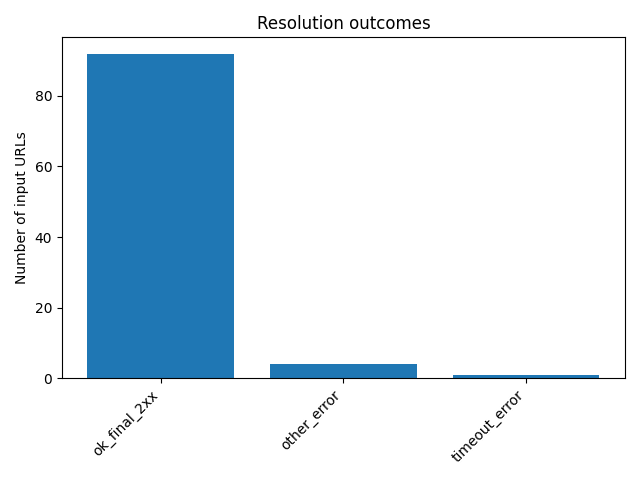
\includegraphics[width=\linewidth]{../results/ca/edu/redirects/resolution_outcomes.png}
% \captionof{figure}{
% This figure shows the distribution of HTTP status codes for the final responses that the scanner received after resolving any redirects. It summarises how often sites eventually returned a success code (2xx), a redirect (3xx), a client error (4xx) such as 404 or 403, or a server error (5xx) such as 500 or 503. In combination with the entry status distribution, it reveals how often a URL ultimately succeeds even if the first response is a redirect or a soft error.
% }
% \label{fig:ca:edu:resolution_outcomes}
% \end{minipage}
% \end{center}

% results from each module. Should also not CA gov standards as an explicity section, then move onto the bonus stuff (e.g., MDN, OWASP)

% Break down the following results per domain (gov, 
    % error_leak
        % - NOTE: Ignore next.js here, lots of false positives
        % what fraction of error pages leaked info
        % what fraction of error pages leaked info about non cloudflare/wordpress/drupal
            % e.g frameworks vs cloud vs servers
        % what fraction had versions 
            % - NOTE: drupal had versions in nearly all of them but the scanner missed drupal specifically
    % hsts/https (CA gov)
        % what percentage redirected http -> https
        % what fraction accepted an http request
        % what fraction actually implemented sts header
    % headers
        % what fraction actually followed best practices (recommended)
        % what fraction contained revealing headers
        % what header's recommendation was most/least abided by.
    % cipher suite/tls (CA gov)
    % any WAF/CDN behaviour observed

% Results structure ideas (facts only):
% - Subsection 1: HTTPS, HSTS, TLS, cipher suites
%   * For CA authorities / CA finance / CA education / CA energy:
%       - % of sites that:
%           · Redirect HTTP→HTTPS for root.
%           · Maintain HTTPS-only (no HTTP listener or always redirect).
%           · Set HSTS, and fraction with "strong" policy (>= 1 year, includeSubDomains).
%       - TLS versions observed: % supporting 1.3, 1.2, % still willing to negotiate 1.0/1.1 (if any).
%       - Cipher posture: % with only modern AEAD suites; % where legacy/weak suites appear in negotiation.
%   * Repeat summary for US and UK comparators by sector.
%
% - Subsection 2: Headers & cookies
%   * Referrer-Policy: fraction with strong defaults vs weaker vs missing.
%   * Clickjacking: % with CSP frame-ancestors and/or X-Frame-Options; note overlaps.
%   * X-Content-Type-Options: nosniff prevalence.
%   * Cookies:
%       - Among sites that set cookies: % using Secure, HttpOnly, and SameSite; count of sites with apparently "session-like" cookies missing flags.
%
% - Subsection 3: CSP, Permissions-Policy, security.txt
%   * CSP: % of sites with any CSP; % with a baseline-protective policy vs extremely permissive (e.g., script-src '*', 'unsafe-inline').
%   * Permissions-Policy: % that set it at all; % with non-trivial deny-lists for powerful features.
%   * security.txt: % with a valid file under /.well-known or /; note common fields present/absent.
%
% - Subsection 4: Error-page behaviour (error_leak module)
%   * For the synthetic missing path:
%       - Status codes: fraction using proper 404/410 vs soft-404 2xx.
%       - Header parity: fraction of sites where error pages "drop" important headers relative to 200s.
%       - Leak patterns: counts for framework banners, full stack traces, file paths, SQL/ORM messages, directory listings.
%   * Note methodological caveat: ignore known Next.js false positives where the "dev style" error pages are benign or mis-classified.
%
% - Subsection 5: WAF/CDN behaviour
%   * Count sites where:
%       - Scanner received immediate 403/503 or "browser check" pages.
%       - Connections consistently timed out / null-routed for all tests.
%   * Report them by sector/jurisdiction as a separate category (not merged into failures).

\subsection{Enough to support main questions}
% RQ coverage:
% - RQ1 (Canadian posture vs baseline):
%   * Use the CA-only numbers for HTTPS, HSTS, TLS versions, cipher strength, cookies, and basic headers.
% - RQ2 (sector/jurisdiction variation):
%   * Tables comparing CA vs US vs UK within each sector for key metrics (HTTPS/HSTS, CSP, security.txt, etc.).
% - RQ3 (second-line defenses and gaps):
%   * Prevalence of CSP, Permissions-Policy, referrer policies, error-page hygiene, security.txt.
%   * WAF/CDN behaviour data (how many sites effectively "opt out" of being measured).


\section{Discussion}\label{sec3}
\subsection{Summary of Results}
% Summary planning:
% - One paragraph per main theme:
%   * Transport-layer: are most public sites on HTTPS with modern TLS or not? Any notable pockets of legacy?
%   * Header/cookie hardening: broadly adopted or patchy? Any sectors standout?
%   * Second-line defenses (CSP, Permissions-Policy, security.txt): still niche or common in certain sectors/jurisdictions?
%   * WAF/CDN: how often our measurement was actively blocked; note that blocking measurement ≠ insecure, but reduces transparency.

 \subsection{Restate \& Answer Main Questions}
 % Answering RQs:
% - RQ1: Conclude whether a typical Canadian public website meets a reasonable minimum baseline (with explicit percentages).
% - RQ2: Highlight clearest cross-sector and cross-country differences (e.g., "finance consistently ahead on TLS/cookies, education lags on security.txt", or whatever your data show).
% - RQ3: Explain where hardening is rare, and what that implies for standards (e.g., CSP and security.txt adoption low despite strong recommendations).

\subsection{Limitations}
% Limitations:
% - Coverage:
%   * Dataset limited to sites that appear in public registries and resolve cleanly; some authorities may use portals under third-party domains.
%   * No deep crawling: results reflect landing pages and a single synthetic error path only.
% - Measurement:
%   * Single vantage point (cloud VM); some behaviours may be geo- or ASN-dependent.
%   * WAF/CDN interference: some results are "unmeasurable" by design.
%   * TLS/cipher behaviour may differ for other SNI/ALPN combinations (e.g., HTTP/2 vs 1.1).
% - Semantics:
%   * Presence of a header does not guarantee correct app-level use (e.g., CSP might be overly permissive).
%   * Stack-trace regexes may miss exotic frameworks or misclassify some verbose messages.
% - Standards interpretation:
%   * "Recommended" vs "required" is a spectrum; you anchored in current guidance but others could choose different thresholds.

\subsection{Conclusion/Recommendation}
% Conclusion & recommendations:
% - For Canadian standards bodies / policymakers:
%   * Consider codifying a clear minimum web security baseline for public-sector sites (HTTPS-only, HSTS, modern TLS, basic hardening headers, security.txt).
%   * Encourage or require regular, automated self-assessment aligned with CCCS and CSA guidance.
% - For site operators:
%   * Practical checklist derived from this study: easiest wins (e.g., HSTS, referrer policy, nosniff, secure cookies) vs more complex items (CSP roll-out, Permissions-Policy).
%   * Suggest incremental adoption paths (e.g., CSP report-only → enforcing; adding security.txt with monitored contact).
% - For the wider community:
%   * Emphasize value of transparent, standards-aligned measurement across jurisdictions and sectors.
\subsection{Future Work}
% Future work:
% - DNS and certificate authority checks (CAA records, OCSP/CRL behaviour) that you deliberately excluded from this phase.
% - Deeper crawling of internal paths and authenticated apps (with appropriate ethics/permissions).
% - Longitudinal measurements to track improvement or regression over time.
% - Extending scanning to additional sectors (healthcare as its own sector, municipal websites, NGOs).
% - Integrating more nuanced WAF detection and collaboration (e.g., whitelisting research scanners).
% - Open-sourcing the tool and encouraging contributions/replications in other countries.

\section{Acknowledgments}\label{sec4}
% Acknowledgments ideas:
% - Funding: CSA Group undergraduate research grant (project name).
% - Institutional support: TRU supervisors/mentors, lab resources.
% - Any assistance with infrastructure (cloud credits, security review, etc.).

\subsection{Funding/Equipment}
\newpage \begin{appendices}\label{app:reproducibility}
\section{Reproducibility Notes}
% Reproducibility notes:
% - Environment:
%   * Python version; key libraries (requests, ssl/PyOpenSSL, etc.).
%   * OS and VM specs.
% - Code:
%   * Repository structure; which commit/tag corresponds to this paper.
%   * High-level configuration: rate limits, timeouts, retry/backoff params.
% - Inputs:
%   * How to reconstruct site lists from the same public sources (without shipping full lists if they are sensitive).
% - Outputs:
%   * What artifacts you can safely share (aggregate stats, per-site anonymised summaries, or full per-site results if approved).
\end{appendices}
\newpage 
% \bibliographystyle{IEEEtranN}
% \bibliography{sn-bibliography}
% \bibliographystyle{sn-mathphys-num}
% \bibliography{sn-bibliography}

\end{document}
